\documentclass[]{article}
\usepackage{lmodern}
\usepackage{amssymb,amsmath}
\usepackage{ifxetex,ifluatex}
\usepackage{fixltx2e} % provides \textsubscript
\ifnum 0\ifxetex 1\fi\ifluatex 1\fi=0 % if pdftex
  \usepackage[T1]{fontenc}
  \usepackage[utf8]{inputenc}
\else % if luatex or xelatex
  \ifxetex
    \usepackage{mathspec}
  \else
    \usepackage{fontspec}
  \fi
  \defaultfontfeatures{Ligatures=TeX,Scale=MatchLowercase}
\fi
% use upquote if available, for straight quotes in verbatim environments
\IfFileExists{upquote.sty}{\usepackage{upquote}}{}
% use microtype if available
\IfFileExists{microtype.sty}{%
\usepackage{microtype}
\UseMicrotypeSet[protrusion]{basicmath} % disable protrusion for tt fonts
}{}
\usepackage[margin=1in]{geometry}
\usepackage{hyperref}
\hypersetup{unicode=true,
            pdftitle={Milestone1},
            pdfauthor={Margot Chen, Qi Yang},
            pdfborder={0 0 0},
            breaklinks=true}
\urlstyle{same}  % don't use monospace font for urls
\usepackage{color}
\usepackage{fancyvrb}
\newcommand{\VerbBar}{|}
\newcommand{\VERB}{\Verb[commandchars=\\\{\}]}
\DefineVerbatimEnvironment{Highlighting}{Verbatim}{commandchars=\\\{\}}
% Add ',fontsize=\small' for more characters per line
\usepackage{framed}
\definecolor{shadecolor}{RGB}{248,248,248}
\newenvironment{Shaded}{\begin{snugshade}}{\end{snugshade}}
\newcommand{\AlertTok}[1]{\textcolor[rgb]{0.94,0.16,0.16}{#1}}
\newcommand{\AnnotationTok}[1]{\textcolor[rgb]{0.56,0.35,0.01}{\textbf{\textit{#1}}}}
\newcommand{\AttributeTok}[1]{\textcolor[rgb]{0.77,0.63,0.00}{#1}}
\newcommand{\BaseNTok}[1]{\textcolor[rgb]{0.00,0.00,0.81}{#1}}
\newcommand{\BuiltInTok}[1]{#1}
\newcommand{\CharTok}[1]{\textcolor[rgb]{0.31,0.60,0.02}{#1}}
\newcommand{\CommentTok}[1]{\textcolor[rgb]{0.56,0.35,0.01}{\textit{#1}}}
\newcommand{\CommentVarTok}[1]{\textcolor[rgb]{0.56,0.35,0.01}{\textbf{\textit{#1}}}}
\newcommand{\ConstantTok}[1]{\textcolor[rgb]{0.00,0.00,0.00}{#1}}
\newcommand{\ControlFlowTok}[1]{\textcolor[rgb]{0.13,0.29,0.53}{\textbf{#1}}}
\newcommand{\DataTypeTok}[1]{\textcolor[rgb]{0.13,0.29,0.53}{#1}}
\newcommand{\DecValTok}[1]{\textcolor[rgb]{0.00,0.00,0.81}{#1}}
\newcommand{\DocumentationTok}[1]{\textcolor[rgb]{0.56,0.35,0.01}{\textbf{\textit{#1}}}}
\newcommand{\ErrorTok}[1]{\textcolor[rgb]{0.64,0.00,0.00}{\textbf{#1}}}
\newcommand{\ExtensionTok}[1]{#1}
\newcommand{\FloatTok}[1]{\textcolor[rgb]{0.00,0.00,0.81}{#1}}
\newcommand{\FunctionTok}[1]{\textcolor[rgb]{0.00,0.00,0.00}{#1}}
\newcommand{\ImportTok}[1]{#1}
\newcommand{\InformationTok}[1]{\textcolor[rgb]{0.56,0.35,0.01}{\textbf{\textit{#1}}}}
\newcommand{\KeywordTok}[1]{\textcolor[rgb]{0.13,0.29,0.53}{\textbf{#1}}}
\newcommand{\NormalTok}[1]{#1}
\newcommand{\OperatorTok}[1]{\textcolor[rgb]{0.81,0.36,0.00}{\textbf{#1}}}
\newcommand{\OtherTok}[1]{\textcolor[rgb]{0.56,0.35,0.01}{#1}}
\newcommand{\PreprocessorTok}[1]{\textcolor[rgb]{0.56,0.35,0.01}{\textit{#1}}}
\newcommand{\RegionMarkerTok}[1]{#1}
\newcommand{\SpecialCharTok}[1]{\textcolor[rgb]{0.00,0.00,0.00}{#1}}
\newcommand{\SpecialStringTok}[1]{\textcolor[rgb]{0.31,0.60,0.02}{#1}}
\newcommand{\StringTok}[1]{\textcolor[rgb]{0.31,0.60,0.02}{#1}}
\newcommand{\VariableTok}[1]{\textcolor[rgb]{0.00,0.00,0.00}{#1}}
\newcommand{\VerbatimStringTok}[1]{\textcolor[rgb]{0.31,0.60,0.02}{#1}}
\newcommand{\WarningTok}[1]{\textcolor[rgb]{0.56,0.35,0.01}{\textbf{\textit{#1}}}}
\usepackage{longtable,booktabs}
\usepackage{graphicx,grffile}
\makeatletter
\def\maxwidth{\ifdim\Gin@nat@width>\linewidth\linewidth\else\Gin@nat@width\fi}
\def\maxheight{\ifdim\Gin@nat@height>\textheight\textheight\else\Gin@nat@height\fi}
\makeatother
% Scale images if necessary, so that they will not overflow the page
% margins by default, and it is still possible to overwrite the defaults
% using explicit options in \includegraphics[width, height, ...]{}
\setkeys{Gin}{width=\maxwidth,height=\maxheight,keepaspectratio}
\IfFileExists{parskip.sty}{%
\usepackage{parskip}
}{% else
\setlength{\parindent}{0pt}
\setlength{\parskip}{6pt plus 2pt minus 1pt}
}
\setlength{\emergencystretch}{3em}  % prevent overfull lines
\providecommand{\tightlist}{%
  \setlength{\itemsep}{0pt}\setlength{\parskip}{0pt}}
\setcounter{secnumdepth}{0}
% Redefines (sub)paragraphs to behave more like sections
\ifx\paragraph\undefined\else
\let\oldparagraph\paragraph
\renewcommand{\paragraph}[1]{\oldparagraph{#1}\mbox{}}
\fi
\ifx\subparagraph\undefined\else
\let\oldsubparagraph\subparagraph
\renewcommand{\subparagraph}[1]{\oldsubparagraph{#1}\mbox{}}
\fi

%%% Use protect on footnotes to avoid problems with footnotes in titles
\let\rmarkdownfootnote\footnote%
\def\footnote{\protect\rmarkdownfootnote}

%%% Change title format to be more compact
\usepackage{titling}

% Create subtitle command for use in maketitle
\providecommand{\subtitle}[1]{
  \posttitle{
    \begin{center}\large#1\end{center}
    }
}

\setlength{\droptitle}{-2em}

  \title{Milestone1}
    \pretitle{\vspace{\droptitle}\centering\huge}
  \posttitle{\par}
    \author{Margot Chen, Qi Yang}
    \preauthor{\centering\large\emph}
  \postauthor{\par}
      \predate{\centering\large\emph}
  \postdate{\par}
    \date{2020/02/27}


\begin{document}
\maketitle

\hypertarget{beijing-pm2.5}{%
\subsection{Beijing PM2.5}\label{beijing-pm2.5}}

\hypertarget{introduction}{%
\subsubsection{Introduction}\label{introduction}}

Beijing, the capital city of China, is fighting against \texttt{PM2.5}
pollution in recent years. \texttt{PM2.5} refers to fine airborne
particles with a diameter of 2.5μm or less. They can cause severe damage
to human health by triggering lung cancer, heart diseases, stroke, and
respiratory infections. A Nature study pointed out that in 2016 only,
\texttt{PM2.5} was associated with over four million deaths worldwide.
In the past decades, the air quality in Beijing has been faced with
great pressure resulting from the rapid development of industry. In
order to secure its citizens' health, Chinese government has taken
action to mitigate the influence of \texttt{PM2.5} since September,
2013.\\
Previous studies showed that \textbf{meteorological conditions}, such as
wind and humidity, could contribute to the formation of \texttt{PM2.5}.
Therefore, we speculate that there could be correlations between
Beijing's \texttt{PM2.5} concentration and the meteorological conditions
in a sufficient period of time. If so, knowing the meteorological
conditions can support the assessment and even prediction of air quality
in Beijing.

\hypertarget{data-description}{%
\subsubsection{Data Description}\label{data-description}}

The
\href{https://archive.ics.uci.edu/ml/datasets/Beijing+PM2.5+Data\#}{dataset}
used in our project was obtained from University of California Irvine
Machine learning Repository. It was originally uploaded by Songxi Chen
in Peking University, China. This is an hourly dataset containing 1) the
\texttt{PM2.5} of US Embassy in Beijing and 2) \textbf{meteorological
statistics} from Beijing Capital International Airport. The data was
collected from Jan 1st, 2010 to Dec 31st, 2014. The original purpose of
the dataset was to assess the effect of Chinese government's pollution
reduction plan which started from September in 2013. The dataset can be
downloaded
\href{https://archive.ics.uci.edu/ml/machine-learning-databases/00381/PRSA_data_2010.1.1-2014.12.31.csv}{here}.

Below are the variables in the dataset:

\begin{longtable}[]{@{}lll@{}}
\toprule
Variable & Type & Description\tabularnewline
\midrule
\endhead
year & Quantitative & Year of data in this row\tabularnewline
month & Quantitative & Month of data in this row\tabularnewline
day & Quantitative & Day of data in this row\tabularnewline
hour & Quantitative & Hour of data in this row\tabularnewline
\texttt{PM2.5} & Quantitative & \texttt{PM2.5} concentration
(ug/m\^{}3)\tabularnewline
DEWP & Quantitative & Dew Point (℃)\tabularnewline
TEMP & Quantitative & Temperature (℃)\tabularnewline
PRES & Quantitative & Pressure (hPa)\tabularnewline
cbwd & Categorical & Combined wind direction\tabularnewline
lws & Quantitative & Cumulated wind speed (m/s)\tabularnewline
ls & Quantitative & Cumulated hours of snow\tabularnewline
lr & Quantitative & Cumulated hours of rain\tabularnewline
\bottomrule
\end{longtable}

\hypertarget{dataset-loading}{%
\subsubsection{Dataset loading}\label{dataset-loading}}

\begin{Shaded}
\begin{Highlighting}[]
\NormalTok{df<-}\KeywordTok{read.csv}\NormalTok{(}\StringTok{"https://archive.ics.uci.edu/ml/machine-learning-databases/00381/PRSA_data_2010.1.1-2014.12.31.csv"}\NormalTok{)}
\end{Highlighting}
\end{Shaded}

\begin{Shaded}
\begin{Highlighting}[]
\KeywordTok{sum}\NormalTok{(}\KeywordTok{is.na}\NormalTok{(df}\OperatorTok{$}\NormalTok{pm2}\FloatTok{.5}\NormalTok{))}\OperatorTok{/}\KeywordTok{length}\NormalTok{(df}\OperatorTok{$}\NormalTok{pm2}\FloatTok{.5}\NormalTok{)}
\end{Highlighting}
\end{Shaded}

\begin{verbatim}
## [1] 0.04716594
\end{verbatim}

So there are 4.73\% missing values in the \texttt{PM2.5} variable, which
shows the data quality is reasonably good. We generated a new dataset
for some plots by omitting the missing values.

\begin{Shaded}
\begin{Highlighting}[]
\NormalTok{df_clean<-}\StringTok{ }\KeywordTok{na.omit}\NormalTok{(df)}
\end{Highlighting}
\end{Shaded}

\hypertarget{dataset-exploration}{%
\subsubsection{Dataset exploration}\label{dataset-exploration}}

\begin{enumerate}
\def\labelenumi{\arabic{enumi}.}
\tightlist
\item
  We are interested in the correlation between meteorological conditions
  (dew point, temperature and pressure) and \texttt{PM2.5}. Thus, we
  created a \textbf{correllogram} of \texttt{DEWP}, \texttt{TEMP},
  \texttt{PRES}, and \texttt{PM2.5}. The graph shows that there each of
  \texttt{DEWP}, \texttt{TEMP}, and \texttt{PRES}could hardly predict
  \texttt{PM2.5}.
\end{enumerate}

\begin{Shaded}
\begin{Highlighting}[]
\NormalTok{df_corr<-}\KeywordTok{cor}\NormalTok{(df_clean[}\DecValTok{6}\OperatorTok{:}\DecValTok{9}\NormalTok{]) }\OperatorTok\StringTok{ }\CommentTok{# get the correlation of the four columns DEWP, TEMP, PRES, and PM2.5 against each other.}
\StringTok{  }\KeywordTok{round}\NormalTok{(}\DecValTok{2}\NormalTok{)}

\KeywordTok{corrplot}\NormalTok{(df_corr,}
         \DataTypeTok{type =} \StringTok{"upper"}\NormalTok{,}
         \DataTypeTok{method =} \StringTok{"color"}\NormalTok{,}
         \DataTypeTok{addCoef.col =} \StringTok{"black"}\NormalTok{,}
         \DataTypeTok{diag =} \OtherTok{FALSE}\NormalTok{)}
\end{Highlighting}
\end{Shaded}

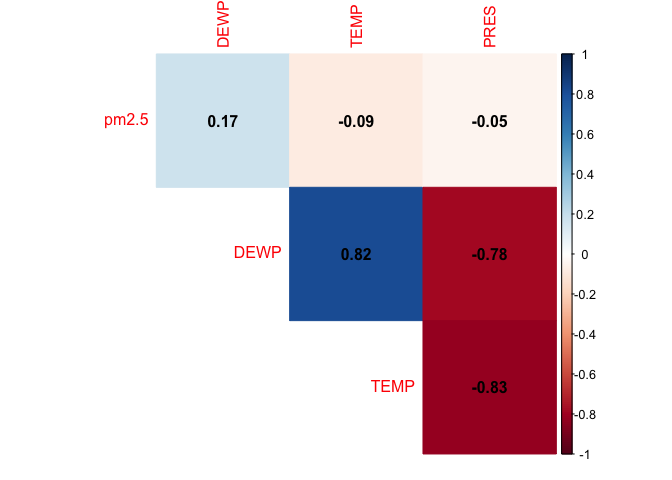
\includegraphics{milestone1_files/figure-latex/unnamed-chunk-4-1.pdf}

\begin{enumerate}
\def\labelenumi{\arabic{enumi}.}
\setcounter{enumi}{1}
\tightlist
\item
  Wind is one of the important elements of weather conditions, and could
  also influence the formation of \texttt{PM2.5}. Therefore, we used a
  \textbf{faceted histogram} in order to check the distribution of
  \texttt{PM2.5} under different wind directions (northwest, northeast,
  southwest and southeast).
\end{enumerate}

\begin{Shaded}
\begin{Highlighting}[]
\NormalTok{df_clean }\OperatorTok\StringTok{ }\KeywordTok{ggplot}\NormalTok{(}\KeywordTok{aes}\NormalTok{(pm2}\FloatTok{.5}\NormalTok{))}\OperatorTok{+}
\StringTok{  }\KeywordTok{geom_histogram}\NormalTok{()}\OperatorTok{+}
\StringTok{  }\KeywordTok{facet_wrap}\NormalTok{(}\OperatorTok{~}\NormalTok{cbwd)}\OperatorTok{+}
\StringTok{  }\KeywordTok{theme_bw}\NormalTok{()}
\end{Highlighting}
\end{Shaded}

\begin{verbatim}
## `stat_bin()` using `bins = 30`. Pick better value with `binwidth`.
\end{verbatim}

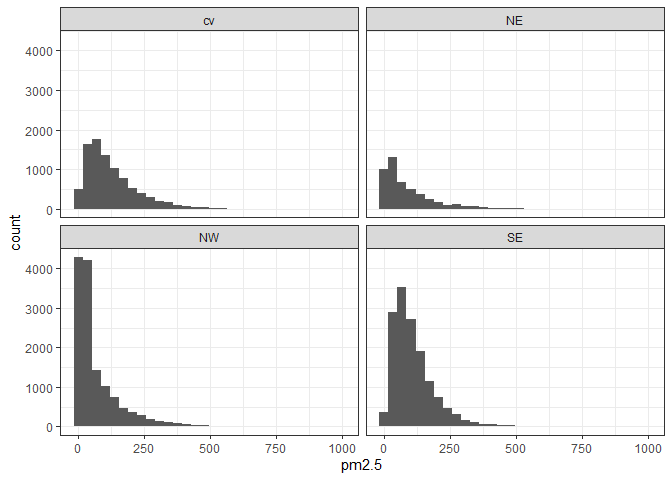
\includegraphics{milestone1_files/figure-latex/unnamed-chunk-5-1.pdf}

\begin{enumerate}
\def\labelenumi{\arabic{enumi}.}
\setcounter{enumi}{2}
\tightlist
\item
  In addition to meteorological conditions, we are curious about the
  potential influence of time on \texttt{PM2.5}, so we created a
  \textbf{heat map} showing \texttt{PM2.5} in different hours and months
  in the year of 2013 and 2014.
\end{enumerate}

\begin{Shaded}
\begin{Highlighting}[]
\CommentTok{# We adopted the code from the following GitHub gist}
\CommentTok{# Title: HeatmapHrByDay.R}
\CommentTok{# Author:  John MacKintosh}
\CommentTok{# Date: Dec 15, 2016}
\CommentTok{# Availability: https://gist.github.com/johnmackintosh/520643a1f82a0c7df00cf949ba98a4e9#file-heatmaphrbyday-r}

\NormalTok{p <-}\StringTok{ }\NormalTok{df }\OperatorTok\StringTok{ }\KeywordTok{filter}\NormalTok{(year}\OperatorTok{>=}\DecValTok{2013}\NormalTok{) }\OperatorTok\StringTok{ }
\StringTok{  }\KeywordTok{ggplot}\NormalTok{(}\KeywordTok{aes}\NormalTok{(day,hour,}\DataTypeTok{fill=}\NormalTok{pm2}\FloatTok{.5}\NormalTok{))}\OperatorTok{+}
\StringTok{  }\KeywordTok{geom_tile}\NormalTok{(}\DataTypeTok{color=} \StringTok{"white"}\NormalTok{,}\DataTypeTok{size=}\FloatTok{0.1}\NormalTok{) }\OperatorTok{+}
\StringTok{  }\KeywordTok{scale_fill_viridis}\NormalTok{(}\DataTypeTok{name=}\StringTok{"Hourly PM2.5"}\NormalTok{, }\DataTypeTok{direction =} \DecValTok{-1}\NormalTok{)}\OperatorTok{+}\StringTok{ }\CommentTok{#Sets the order of colours in the scale reverse}
\StringTok{  }\KeywordTok{facet_grid}\NormalTok{(year}\OperatorTok{~}\NormalTok{month)}\OperatorTok{+}
\StringTok{  }\KeywordTok{scale_y_continuous}\NormalTok{(}\DataTypeTok{trans =} \StringTok{"reverse"}\NormalTok{, }\DataTypeTok{breaks =} \KeywordTok{unique}\NormalTok{(df}\OperatorTok{$}\NormalTok{hour))}\OperatorTok{+}
\StringTok{  }\KeywordTok{scale_x_continuous}\NormalTok{(}\DataTypeTok{breaks =}\KeywordTok{c}\NormalTok{(}\DecValTok{1}\NormalTok{,}\DecValTok{10}\NormalTok{,}\DecValTok{20}\NormalTok{,}\DecValTok{31}\NormalTok{))}\OperatorTok{+}
\StringTok{  }\KeywordTok{theme_minimal}\NormalTok{(}\DataTypeTok{base_size =} \DecValTok{8}\NormalTok{)}\OperatorTok{+}
\StringTok{  }\KeywordTok{labs}\NormalTok{(}\DataTypeTok{title=} \StringTok{"Hourly PM2.5"}\NormalTok{, }\DataTypeTok{x=}\StringTok{"Day"}\NormalTok{, }\DataTypeTok{y=}\StringTok{"Hour"}\NormalTok{)}\OperatorTok{+}
\StringTok{  }\KeywordTok{theme}\NormalTok{(}\DataTypeTok{legend.position =} \StringTok{"bottom"}\NormalTok{)}

\NormalTok{p}
\end{Highlighting}
\end{Shaded}

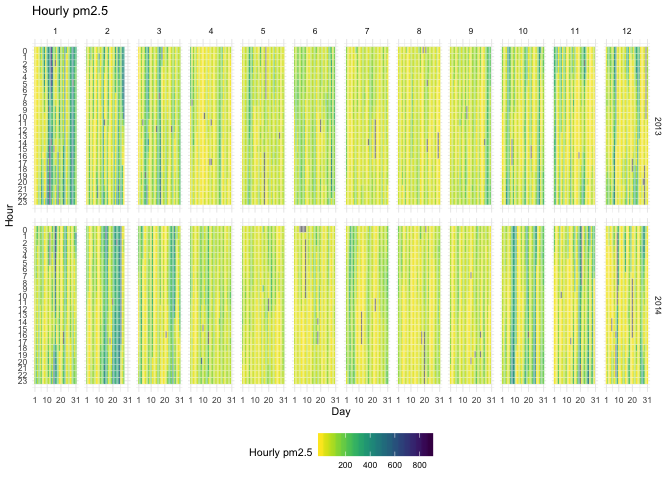
\includegraphics{milestone1_files/figure-latex/unnamed-chunk-6-1.pdf}

\begin{enumerate}
\def\labelenumi{\arabic{enumi}.}
\setcounter{enumi}{3}
\tightlist
\item
  We also create a \textbf{histogram} emphasizing the severity of
  \texttt{PM2.5} in different seasons. We can see from the graph that
  autumn and winter tend to have the most severe \texttt{PM2.5}
  pollution.
\end{enumerate}

\begin{Shaded}
\begin{Highlighting}[]
\NormalTok{df_hist <-}\StringTok{ }\NormalTok{df_clean }\OperatorTok\StringTok{ }
\StringTok{  }\KeywordTok{mutate}\NormalTok{(}\DataTypeTok{season =} \KeywordTok{case_when}\NormalTok{(month }\OperatorTok{==}\StringTok{ }\DecValTok{12} \OperatorTok{~}\StringTok{ 'Winter'}\NormalTok{, month }\OperatorTok{>=}\StringTok{ }\DecValTok{9} \OperatorTok{~}\StringTok{ 'Autumn'}\NormalTok{, month }\OperatorTok{>=}\StringTok{ }\DecValTok{6} \OperatorTok{~}\StringTok{ 'Summer'}\NormalTok{, month }\OperatorTok{>=}\StringTok{ }\DecValTok{3} \OperatorTok{~}\StringTok{ 'Spring'}\NormalTok{,}\OtherTok{TRUE} \OperatorTok{~}\StringTok{ 'Winter'}\NormalTok{))  }\CommentTok{# Group dates to seasons}
\NormalTok{df_hist =}\StringTok{ }\KeywordTok{aggregate}\NormalTok{(df_hist}\OperatorTok{$}\NormalTok{pm2}\FloatTok{.5}\NormalTok{,}
                \DataTypeTok{by =} \KeywordTok{list}\NormalTok{(df_hist}\OperatorTok{$}\NormalTok{season),}
                \DataTypeTok{FUN =}\NormalTok{ mean) }\CommentTok{# Mean [PM2.5] of each season}
\NormalTok{df_hist =}\StringTok{ }\KeywordTok{rename}\NormalTok{(df_hist, }\KeywordTok{c}\NormalTok{(}\StringTok{"season"}\NormalTok{ =}\StringTok{ "Group.1"}\NormalTok{, }\StringTok{"PM2.5"}\NormalTok{ =}\StringTok{ "x"}\NormalTok{)) }
\NormalTok{(season_pmconc <-}\StringTok{ }\KeywordTok{ggplot}\NormalTok{(}\DataTypeTok{data =}\NormalTok{ df_hist, }\KeywordTok{aes}\NormalTok{(}\DataTypeTok{x=}\NormalTok{season, }\DataTypeTok{y =}\NormalTok{ PM2}\FloatTok{.5}\NormalTok{)) }\OperatorTok{+}
\StringTok{  }\KeywordTok{geom_bar}\NormalTok{(}\DataTypeTok{stat=}\StringTok{"identity"}\NormalTok{)}\OperatorTok{+}
\StringTok{  }\KeywordTok{coord_cartesian}\NormalTok{(}\DataTypeTok{ylim=}\KeywordTok{c}\NormalTok{(}\DecValTok{80}\NormalTok{,}\DecValTok{120}\NormalTok{))}\OperatorTok{+}
\StringTok{  }\KeywordTok{labs}\NormalTok{(}\DataTypeTok{x =} \StringTok{"Season"}\NormalTok{, }
       \DataTypeTok{y =} \StringTok{"[PM2.5]"}\NormalTok{,}
       \DataTypeTok{title =} \StringTok{"PM2.5 VS Season"}\NormalTok{) }\OperatorTok{+}
\StringTok{  }\KeywordTok{theme_classic}\NormalTok{()) }
\end{Highlighting}
\end{Shaded}

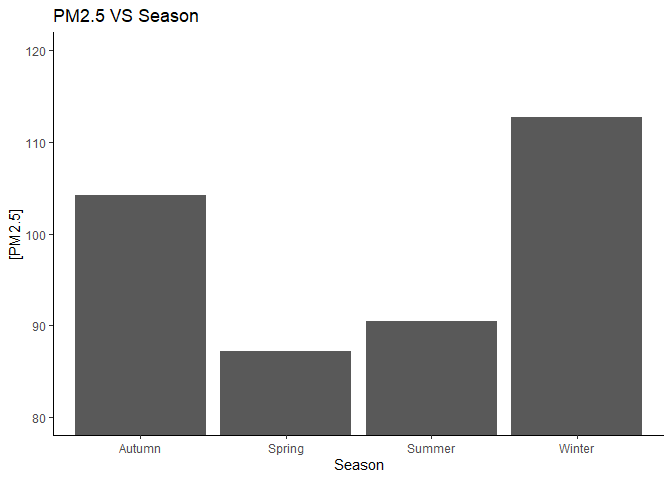
\includegraphics{milestone1_files/figure-latex/unnamed-chunk-7-1.pdf}

\begin{enumerate}
\def\labelenumi{\arabic{enumi}.}
\setcounter{enumi}{4}
\tightlist
\item
  In order to check the effect of \texttt{PM2.5} reduction plan
  initiated by Chinese government in September, 2013, we generated a
  \textbf{line chart} showing how \texttt{PM2.5} changes across time.
  The \texttt{PM2.5} concentration seems to fluctuate, and there is no
  significant drop from 2010 to 2014.
\end{enumerate}

\begin{Shaded}
\begin{Highlighting}[]
\NormalTok{df_year_change <-}\StringTok{ }\NormalTok{df_clean}
\NormalTok{df_year_change}\OperatorTok{$}\NormalTok{date =}\StringTok{ }\KeywordTok{as.Date}\NormalTok{(}\KeywordTok{with}\NormalTok{(df_year_change, }\KeywordTok{paste}\NormalTok{(year, month, day,}\DataTypeTok{sep=}\StringTok{"-"}\NormalTok{)), }\StringTok{"%Y-%m-%d"}\NormalTok{) }\CommentTok{# Combine day, month and year to date}
\NormalTok{df_year_change =}\StringTok{ }\KeywordTok{aggregate}\NormalTok{(df_year_change}\OperatorTok{$}\NormalTok{pm2}\FloatTok{.5}\NormalTok{,}
                \DataTypeTok{by =} \KeywordTok{list}\NormalTok{(df_year_change}\OperatorTok{$}\NormalTok{date),}
                \DataTypeTok{FUN =}\NormalTok{ mean) }\CommentTok{# Mean [PM2.5] of each date}
\NormalTok{df_year_change =}\StringTok{ }\KeywordTok{rename}\NormalTok{(df_year_change, }\KeywordTok{c}\NormalTok{(}\StringTok{"date"}\NormalTok{ =}\StringTok{ "Group.1"}\NormalTok{, }\StringTok{"PM2.5"}\NormalTok{=}\StringTok{"x"}\NormalTok{))}
\NormalTok{(}\DataTypeTok{year_conc =} \KeywordTok{ggplot}\NormalTok{(}\DataTypeTok{data =}\NormalTok{ df_year_change) }\OperatorTok{+}
\StringTok{  }\KeywordTok{geom_line}\NormalTok{(}\KeywordTok{aes}\NormalTok{(}\DataTypeTok{x=}\NormalTok{date, }\DataTypeTok{y=}\NormalTok{PM2}\FloatTok{.5}\NormalTok{), }
            \DataTypeTok{alpha =} \FloatTok{0.6}\NormalTok{,}
            \DataTypeTok{size =} \FloatTok{0.6}\NormalTok{) }\OperatorTok{+}
\StringTok{  }\KeywordTok{geom_vline}\NormalTok{(}\DataTypeTok{xintercept =} \KeywordTok{as.numeric}\NormalTok{(}\KeywordTok{as.Date}\NormalTok{(}\StringTok{"2013-09-01"}\NormalTok{)), }\DataTypeTok{linetype=}\DecValTok{4}\NormalTok{, }\DataTypeTok{color =} \StringTok{"blue"}\NormalTok{, }\DataTypeTok{size =} \DecValTok{1}\NormalTok{)}\OperatorTok{+}
\StringTok{  }\KeywordTok{labs}\NormalTok{(}\DataTypeTok{x =} \StringTok{"Time"}\NormalTok{, }
       \DataTypeTok{y =} \StringTok{"[PM2.5]"}\NormalTok{,}
       \DataTypeTok{title =} \StringTok{"[PM2.5] VS Time"}\NormalTok{) }\OperatorTok{+}
\StringTok{  }\KeywordTok{theme_classic}\NormalTok{())}
\end{Highlighting}
\end{Shaded}

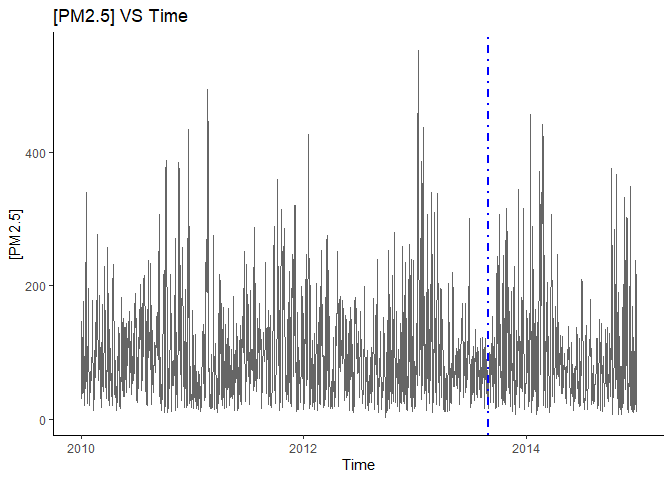
\includegraphics{milestone1_files/figure-latex/unnamed-chunk-8-1.pdf}

\begin{Shaded}
\begin{Highlighting}[]
\NormalTok{?geom_vline}
\end{Highlighting}
\end{Shaded}

\begin{verbatim}
## starting httpd help server ... done
\end{verbatim}

\hypertarget{research-question}{%
\subsubsection{Research Question}\label{research-question}}

Our main research question is an \emph{exploratory} question: does the
\texttt{PM2.5} in Beijing correlates with meteorological conditions and
time? Sub-questions as below are also \emph{exploratory} as they all
focus on the correlation between \texttt{PM2.5} and a certain
variable.\\
- \texttt{PM2.5} VS. physical parameters (dew point, temperature and
pressure).\\
- \texttt{PM2.5} VS. wind.\\
- \texttt{PM2.5} VS. special weather conditions (rain and snow).\\
- \texttt{PM2.5} VS. time (year, month, a time in a day).

\hypertarget{plan-of-action}{%
\subsubsection{Plan of Action}\label{plan-of-action}}

\begin{enumerate}
\def\labelenumi{\arabic{enumi}.}
\tightlist
\item
  Deal with missing values.
\item
  Run tests of correlation between \texttt{PM2.5} and meteorological
  statistics/time.
\item
  Perform a linear regression analyses and plot quantitative variables
  in a regression line.
\item
  Demonstrate the correlation between \texttt{PM2.5} and categorical
  variables. Only wind direction is a categorical variable at first, but
  categorical time units (season, day or night) can also be adapted from
  quantitative records.
\item
  Create an interactive dashboard showing potential correlations between
  meteorological conditions/time and \texttt{PM2.5}.
\item
  Address the effectiveness of Chinese government's action on solving
  air quality issues.
\end{enumerate}

\hypertarget{references}{%
\subsubsection{References}\label{references}}

Liang, X., Zou, T., Guo, B., Li, S., Zhang, H., Zhang, S., Huang, H. and
Chen, S. X. (2015). Assessing Beijing's PM2.5 pollution: severity,
weather impact, APEC and winter heating. Proceedings of the Royal
Society A, 471, 20150257.


\end{document}
